\documentclass[12pt]{article}
\usepackage{geometry}
\geometry{margin=1in}
\usepackage{graphicx}
\usepackage{listings}
\usepackage{xcolor}
\usepackage{hyperref}
\hypersetup{
    colorlinks=true,
    linkcolor=blue,
    filecolor=magenta,
    urlcolor=cyan,
    pdftitle={Yelp Database Analysis},
    pdfpagemode=FullScreen,
}
\lstset{
    basicstyle=\ttfamily\footnotesize,
    keywordstyle=\color{blue},
    stringstyle=\color{red},
    commentstyle=\color{green!60!black},
    backgroundcolor=\color{gray!10},
    breaklines=true,
    frame=single,
    numbers=left,
    numberstyle=\tiny\color{gray},
    captionpos=b,
}
\title{PostgreSQL and MongoDB Query Analysis on Yelp Dataset}
\author{Kartikeya Sharma, Clement Lui, Richard Villagomez, Nicholas Chae}
\date{\today}
\begin{document}

\maketitle

\section{Dataset Selection}
The Yelp dataset was chosen due to its comprehensive structure, which includes user profiles, business details, and reviews. It offers diverse use cases for benchmarking relational (PostgreSQL) and non-relational (MongoDB) database systems.

\subsection{Dataset Details}
The Yelp dataset consists of:
\begin{itemize}
    \item \textbf{Businesses:} Name, location, attributes (e.g., parking, WiFi).
    \item \textbf{Reviews:} User-generated text reviews, ratings, and interaction metrics.
    \item \textbf{Users:} User profiles with review history and friend lists.
\end{itemize}


We selected the \href{https://www.yelp.com/dataset}{Yelp Open Dataset}, a 8.65 GB dataset which contains a subset of businesses, user data, and reviews provided as JSON files. The dataset is made up of 6,990,280 reviews, 150,346 businesses, and 200,100 pictures (not utilized in our project) from 11 metropolitan areas. Over 1.2 million business attributes are accessible along with 908,915 tips (quick suggestions) from 1,987,897 users.

\begin{figure}[h!]
    \centering
    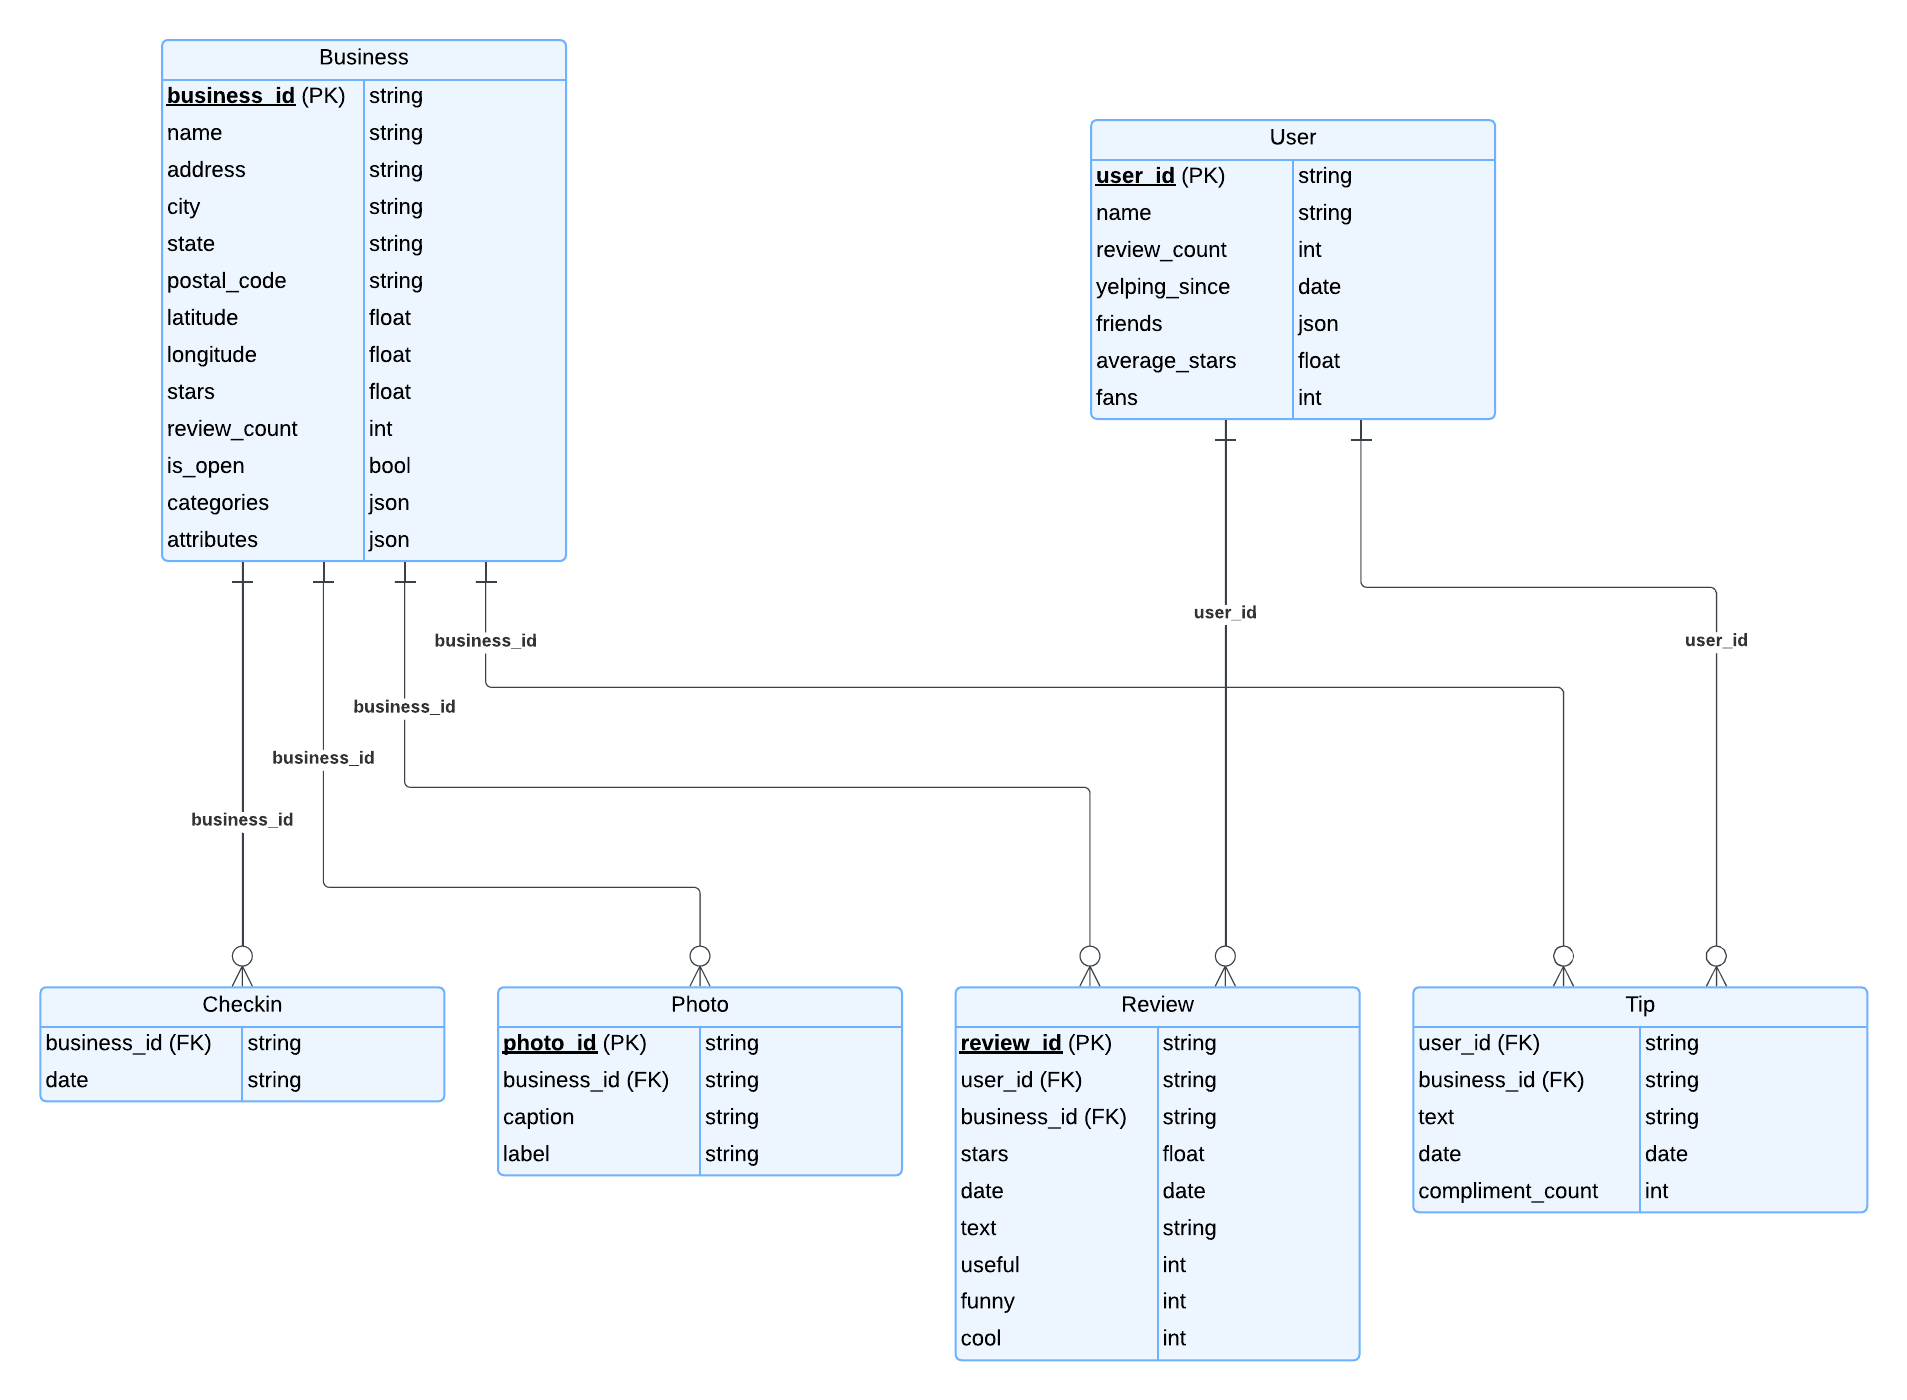
\includegraphics[width=0.8\textwidth]{er-diagram.png} % Change 'image.png' to your image file name
    \caption{ER diagram of Yelp dataset schema and relationships.}
    \label{fig:example} % Label for referencing the figure in the text
\end{figure}


As seen in our ER diagram, the dataset is made up of the following JSON files:
\begin{itemize}
    \item \textbf{business.json}: Business data, location data, attributes, and categories.
    \item \textbf{review.json}: Review text data, \texttt{user\_id} of the review writer, \texttt{business\_id} of the business reviewed, and review attributes and votes.
    \item \textbf{user.json}: User data, attributes, user friend mapping, user metadata.
    \item \textbf{checkin.json}: \texttt{business\_id}, date of check-in.
    \item \textbf{tip.json}: Tip text data, \texttt{user\_id} and \texttt{business\_id}.
    \item \textbf{photo.json}: Photo and \texttt{business\_ids}, photo attributes.
\end{itemize}

Each file is composed of a single object type, one JSON-object per line.


\section{Data Sampling and Truncation Setup}

The Yelp dataset is comprehensive, encompassing millions of records across users, businesses, and reviews. To ensure efficient processing while maintaining representativeness, we applied the following sampling and truncation strategies:

\begin{itemize}
    \item \textbf{Users:} The dataset originally contains several million user records. We sampled approximately 2 million users to reduce storage overhead and computational complexity. This sampling ensures proportional representation across different user activity levels and geographies.
    \item \textbf{Businesses:} All business records were retained without sampling. This allows for a complete representation of businesses across regions and categories.
    \item \textbf{Reviews:} Reviews were filtered based on references to existing users in the \texttt{users} table and businesses in the \texttt{businesses} table. This ensures referential integrity while excluding reviews that belong to users or businesses outside our database.
\end{itemize}

\subsection{Sampled data statistics (as a comparative table):}


\section{Database Loading and System Setup}

\subsection*{PostgreSQL Setup}
Data was transformed from JSON to CSV using Python for bulk insertion into PostgreSQL.

\textbf{Steps:}
\begin{enumerate}
    \item Installed PostgreSQL 14 locally using \texttt{brew install postgresql@14}.
    \item Created tables for users, businesses, and reviews.
    \item Used the \texttt{COPY} command for efficient bulk data insertion.
\end{enumerate}

\textbf{Code Snippet:}
\begin{lstlisting}[language=Python, caption=Loading Users into PostgreSQL]
import json
import psycopg

# Connect to PostgreSQL
conn = psycopg.connect("dbname=yelp user=jadoo")
cur = conn.cursor()

# Create the reviews table if it doesn't exist
cur.execute("""
    CREATE TABLE IF NOT EXISTS reviews (
        review_id TEXT PRIMARY KEY,
        user_id TEXT REFERENCES users(user_id),
        business_id TEXT REFERENCES business(business_id),
        stars FLOAT,
        text TEXT,
        useful INT,
        funny INT,
        cool INT,
        date TIMESTAMP
    );
""")
conn.commit()

# Load reviews from JSON and insert into the database
file_path = "../data/yelp_academic_dataset_review.json"
batch_size = 1000
batch = []

with open(file_path, "r", encoding="utf-8") as f:
    for line in f:
        review = json.loads(line)

        # Check if user_id and business_id exist
        cur.execute("""
            SELECT EXISTS (
                SELECT 1 FROM users WHERE user_id = %s
            ) AND EXISTS (
                SELECT 1 FROM business WHERE business_id = %s
            );
        """, (review["user_id"], review["business_id"]))
        exists = cur.fetchone()[0]

        # Add to batch if both foreign keys are valid
        if exists:
            batch.append((
                review["review_id"],
                review["user_id"],
                review["business_id"],
                review["stars"],
                review["text"],
                review["useful"],
                review["funny"],
                review["cool"],
                review["date"]
            ))


# Insert remaining records
if batch:
    cur.executemany("""
        INSERT INTO reviews (review_id, user_id, business_id, stars, text, useful, funny, cool, date)
        VALUES (%s, %s, %s, %s, %s, %s, %s, %s, %s)
        ON CONFLICT (review_id) DO NOTHING;
    """, batch)
    conn.commit()

cur.close()
conn.close()
print("Reviews data loaded successfully!")

\end{lstlisting}

\subsection{Handling Data Conflicts}

When inserting review data, the \texttt{ON CONFLICT} clause was applied to the \texttt{review\_id} column, which is the primary key of the \texttt{reviews} table. This ensured that any duplicate entries in the JSON dataset were automatically skipped without disrupting the migration process. The \texttt{ON CONFLICT} clause prevented errors by instructing PostgreSQL to \textit{do nothing} when a conflict was detected on the \texttt{review\_id} key. Below is the relevant code snippet:

\begin{lstlisting}[language=Python, caption={Batch Insert with Conflict Handling in PostgreSQL}]
# Insert batch into the database
if len(batch) >= batch_size:
    cur.executemany("""
        INSERT INTO reviews (review_id, user_id, business_id, stars, text, useful, funny, cool, date)
        VALUES (%s, %s, %s, %s, %s, %s, %s, %s, %s)
        ON CONFLICT (review_id) DO NOTHING;
    """, batch)
    conn.commit()
    batch = []
\end{lstlisting}



\subsection*{MongoDB Setup}
MongoDB's document-based structure allowed for direct ingestion of JSON data.

\textbf{Steps:}
\begin{enumerate}
    \item Installed MongoDB locally.
    \item Used Python's \texttt{pymongo} library to insert JSON data directly.
    \item Created separate collections for users, businesses, and reviews.
\end{enumerate}

\textbf{Code Snippet:}
\begin{lstlisting}[language=Python, caption=Loading Data into MongoDB]
from pymongo import MongoClient
import json

client = MongoClient("mongodb://localhost:27017/")
db = client["yelp"]

with open("yelp_academic_dataset_business.json", "r") as f:
    businesses = [json.loads(line) for line in f]
db.businesses.insert_many(businesses)
\end{lstlisting}

\textbf{Observations:}
\begin{itemize}
    \item MongoDB's flexibility significantly simplified the loading process compared to PostgreSQL.
    \item PostgreSQL required schema definition and data transformation, whereas MongoDB allowed direct ingestion of JSON.
\end{itemize}

\section{Benchmark Queries}
Before starting, we would like remark that although all Postgres queries are analyzed using "EXPLAIN ANALYZE" and similarly using ".explain()" for MongoDB queries, we decided not to include them in all of our queries since they take a lot of unnecessary space. They are included in the .ipynb on GitHub.

\subsection*{Task 1: Aggregate Analysis on Business Data}

Analyze the distribution of user activity by finding how many reviews users typically post. This involves grouping users by their total number of reviews and counting the number of users in each group.


\textbf{Query (PostgreSQL):}
\begin{lstlisting}[language=SQL, caption=Aggregate]
SELECT 
    num_reviews,
    COUNT(*) AS num_users
FROM (
    SELECT 
        r.user_id,
        COUNT(r.review_id) AS num_reviews
    FROM 
        reviews r
    GROUP BY 
        r.user_id
) AS user_review_counts
GROUP BY 
    num_reviews
ORDER BY 
    num_reviews DESC;

\end{lstlisting}

\textbf{Query (MongoDB):}
\begin{lstlisting}[language=python]
pipeline = [
    {
        "$group": {
            "_id": "$user_id",  # Group by user_id
            "num_reviews": {"$count": {}}  # Count reviews per user
        }
    },
    {
        "$group": {
            "_id": "$num_reviews",  # Group by the count of reviews
            "num_users": {"$sum": 1}  # Count users with that many reviews
        }
    },
    {
        "$sort": {"_id": -1}  # Sort by number of reviews in descending order
    }
]

# Execute the pipeline
results = list(db.reviews.aggregate(pipeline))
\end{lstlisting}


\textbf{PostgreSQL:}
\begin{itemize}
\item Time: About 13.2 s
\item Strength: The declarative SQL syntax allows for concise and logical query structuring, especially with nested queries.
\item Weakness: Data loading was slower due to strict schema adherence and bulk insert operations.
\item PostgreSQL offered superior indexing and query performance.
\end{itemize}

\begin{lstlisting}[caption={Execution Plan}]
Sort  (cost=975139.25..975139.75 rows=200 width=16) (actual time=13608.040..13637.559 rows=565 loops=1)
  Sort Key: (count(r.review_id)) DESC
  Sort Method: quicksort  Memory: 51kB
  ->  HashAggregate  (cost=975129.61..975131.61 rows=200 width=16) (actual time=13607.904..13637.441 rows=565 loops=1)
        Group Key: count(r.review_id)
        Batches: 1  Memory Usage: 121kB
        ->  Finalize GroupAggregate  (cost=914306.02..971729.74 rows=226658 width=31) (actual time=12964.924..13539.277 rows=1929782 loops=1)
              Group Key: r.user_id
              ->  Gather Merge  (cost=914306.02..967196.58 rows=453316 width=31) (actual time=12964.913..13310.578 rows=2933023 loops=1)
                    Workers Planned: 2
                    Workers Launched: 2
                    ->  Sort  (cost=913306.00..913872.64 rows=226658 width=31) (actual time=12945.696..13036.138 rows=977674 loops=3)
                          Sort Key: r.user_id
                          Sort Method: external merge  Disk: 40032kB
                          Worker 0:  Sort Method: external merge  Disk: 40496kB
                          Worker 1:  Sort Method: external merge  Disk: 40144kB
                          ->  Partial HashAggregate  (cost=836319.76..887719.59 rows=226658 width=31) (actual time=12043.941..12670.398 rows=977674 loops=3)
                                Group Key: r.user_id
                                Planned Partitions: 16  Batches: 85  Memory Usage: 4753kB  Disk Usage: 145976kB
                                Worker 0:  Batches: 89  Memory Usage: 4753kB  Disk Usage: 146136kB
                                Worker 1:  Batches: 89  Memory Usage: 4753kB  Disk Usage: 145952kB
                                ->  Parallel Seq Scan on reviews r  (cost=0.00..569908.36 rows=2795136 width=46) (actual time=0.173..10705.123 rows=2233667 loops=3)
Planning Time: 5.372 ms
Execution Time: 13653.087 ms
\end{lstlisting}

\subsubsection*{Execution Summary}
\begin{itemize}
    \item \textbf{Total Execution Time:} 13653.087 ms.
    \item \textbf{Sort Method:} Quicksort, using 51kB of memory.
    \item \textbf{Parallel Execution:} Involved 2 workers for parallel sequence scans.
    \item \textbf{Disk Usage:} External merge required disk usage of approximately 40MB per worker.
    \item \textbf{Group Aggregate:} Hash aggregation used memory and disk efficiently, with 85 partitions and 145MB disk usage per worker.
\end{itemize}


\textbf{MongoDB:}
\begin{itemize}
\item \textbf{Total Execution Time:} About 23.18 s
\item \textbf{Strength: } The aggregation pipeline simplifies operations for semi-structured data, especially when fields are nested.
\item \textbf{Strength:} Data loading was simpler and faster due to its schema-less nature.
\item \textbf{Weakness:} The lack of built-in indexing during initial queries caused slower execution times for the first run.
\item \textbf{Aggregation: }MongoDB’s aggregation pipeline was easier to write for semi-structured data.
\end{itemize}



\subsection*{Task 2: Keyword Search in Reviews}
Search for reviews containing the word “horrible” in the text field, and count. \newline

\textbf{Query (PostgreSQL):}
\begin{lstlisting}[language=SQL]
SELECT COUNT(*) AS review_count
FROM reviews
WHERE text ILIKE '%horrible%'
\end{lstlisting}

\textbf{Query (MongoDB):}
\begin{lstlisting}[language=python]
# Define the word to search for
word_to_search = "horrible"

# Use an aggregation pipeline to count matching reviews
pipeline = [
    {"$match": {"text": {"$regex": word_to_search, "$options": "i"}}},  # Case-insensitive regex match
    {"$count": "review_count"}  # Count the number of matching documents
]

# Run the aggregation pipeline
result = list(db.reviews.aggregate(pipeline))
\end{lstlisting}

\newpage

\textbf{PostgreSQL:}
\begin{itemize}
    \item \textbf{Total Execution Time:} 6.974 ms
    \item \textbf{Query Plan:}
        \begin{itemize}
            \item \textbf{Seq Scan:} Performed a sequential scan on the \texttt{reviews} table.
            \item \textbf{Filter:} Applied a case-insensitive pattern match on the \texttt{text} column using the \texttt{ILIKE} operator.
        \end{itemize}
    \item \textbf{Planning Time:} 7.179 ms
    \item \textbf{Strength:} 
        \begin{itemize}
            \item Efficient for structured datasets with predefined schemas.
            \item Ability to use complex SQL operations for data analysis.
        \end{itemize}
    \item \textbf{Weakness:} Performance may degrade on very large datasets without proper indexing.
\end{itemize}

\textbf{MongoDB:}
\begin{itemize}
    \item \textbf{Total Execution Time:} 23.18 s
    \item \textbf{Query Plan:}
        \begin{itemize}
            \item \textbf{Stage:} \texttt{COLLSCAN} (Collection Scan).
            \item \textbf{Filter:} Applied a case-insensitive regex filter on the \texttt{text} field.
        \end{itemize}
    \item \textbf{Strength:} Aggregation pipeline is easier to write for semi-structured data.
    \item \textbf{Weakness:} Without proper indexing, queries can result in slow performance due to collection scans.
\end{itemize}

\subsection*{Task 3: Top Categories by Average Rating}

\textbf{Query (PostgreSQL)}
\begin{lstlisting}[language=SQL, caption=Query to find top categories by average rating]
SELECT 
    category,
    AVG(b.stars) AS average_rating,
    COUNT(b.business_id) AS num_businesses
FROM (
    SELECT 
        business_id,
        UNNEST(STRING_TO_ARRAY(categories, ', ')) AS category,
        stars
    FROM business
) b
GROUP BY category
ORDER BY average_rating DESC
LIMIT 20;
\end{lstlisting}

\subsubsection*{Result:}
\begin{table}[h!]
\centering
\begin{tabular}{|l|c|c|}
\hline
\textbf{Category} & \textbf{Average Rating} & \textbf{Number of Businesses} \\
\hline
Cheese Tasting Classes & 5.0 & 2 \\
Silent Disco & 5.0 & 2 \\
Experiences & 5.0 & 2 \\
Water Suppliers & 5.0 & 1 \\
Art Consultants & 5.0 & 2 \\
Childproofing & 5.0 & 3 \\
Patent Law & 5.0 & 1 \\
Mohels & 5.0 & 1 \\
Karaoke Rental & 5.0 & 1 \\
Bubble Soccer & 5.0 & 1 \\
Metal Detector Services & 5.0 & 1 \\
Somali & 5.0 & 2 \\
Circus Schools & 5.0 & 1 \\
Sport Equipment Hire & 5.0 & 1 \\
Calligraphy & 5.0 & 2 \\
Real Estate Photography & 4.90625 & 32 \\
Undersea/Hyperbaric Medicine & 4.9 & 5 \\
Gerontologists & 4.875 & 4 \\
Art Tours & 4.8611 & 18 \\
Boudoir Photography & 4.8378 & 37 \\
\hline
\end{tabular}
\caption{Top 10 Categories by Average Rating}
\label{tab:top_categories}
\end{table}

\textbf{Query (MongoDB):}
\begin{lstlisting}[language=python]
# Define the aggregation pipeline
pipeline = [
    # Stage 1: Split categories into an array
    {
        "$project": {
            "business_id": 1,
            "stars": 1,
            "categories": {
                "$split": ["$categories", ", "]
            }
        }
    },
    # Stage 2: Unwind the categories array
    {
        "$unwind": "$categories"
    },
    # Stage 3: Group by category to calculate the average rating and count
    {
        "$group": {
            "_id": "$categories",
            "average_rating": {"$avg": "$stars"},
            "num_businesses": {"$sum": 1}
        }
    },
    # Stage 4: Sort by average rating in descending order
    {
        "$sort": {"average_rating": -1}
    },
    # Stage 5: Limit to top 10 categories
    {
        "$limit": 20
    }
]

# Execute the pipeline
results = list(db.business.aggregate(pipeline))
for result in results:
    print(result)

\end{lstlisting}

\subsection*{Task 4: }
\textbf{Query (PostgreSQL):}
\begin{lstlisting}[language=SQL]
SELECT 
\end{lstlisting}

\textbf{Query (MongoDB):}
\begin{lstlisting}[language=python]

\end{lstlisting}

\subsection*{Task 5: }
\textbf{Query (PostgreSQL):}
\begin{lstlisting}[language=SQL]
SELECT 
\end{lstlisting}

\textbf{Query (MongoDB):}
\begin{lstlisting}[language=python]

\end{lstlisting}

\section{Reflections}

\end{document}

